%%%administrators guide for libpniutils

\documentclass[a4paper,twoside]{book}
\usepackage{a4wide,amsmath,graphics}
\usepackage{listings}
\usepackage{float}
\usepackage{hyperref}
\author{Eugen Wintersberger}
\title{{\Huge libpninx\\ Users guide}}

%%setup the listings package
\lstset{language=C++}
\lstdefinestyle{numbers}{numbers=left,stepnumber=1,numberstyle=\small}
\lstset{style=numbers}
\lstset{captionpos=b,frame=lines,float=tb}
\lstset{floatplacement=tb}
\lstset{basicstyle=\small}
\lstset{tabsize=2}

%%%setup for hyperref
\hypersetup{pdftitle=libpninx Users Guide,
                pdfborder=0 0 0,
                colorlinks=false}

%%define some custom commands
\newcommand{\pninx}{{\tt libpninx}}
\newcommand{\nxfield}{{\tt NXField}}
\newcommand{\nxobject}{{\tt NXObject}}
\newcommand{\nxfile}{{\tt NXFile}}
\newcommand{\nxgroup}{{\tt NXGroup}}
\newcommand{\nxnumericfield}{{\tt NXNumericField}}
\newcommand{\nxstringfield}{{\tt NXStringField}}
\newcommand{\nxbinaryfield}{{\tt NXBinaryField}}
\newcommand{\arrayt}{{\tt Array<>}}
\newcommand{\scalart}{{\tt Scalar<>}}
\newcommand{\pniutils}{{\tt libpniutils}}

%%%setup custom chapter header 
\floatstyle{ruled}
\newfloat{mylistings}{htb}{lop}[chapter]

\makeatletter
\renewcommand{\@makechapterhead}[1]{%
\vspace*{50 pt}%
{\setlength{\parindent}{0pt} \raggedright \normalfont
\bfseries\Huge
\ifnum \value{secnumdepth}>1 
   \if@mainmatter\thechapter.\ \fi%
\fi
#1\par\nobreak\vspace{40 pt}}}
\makeatother
%%------------------------------------------

\begin{document}
\maketitle
\tableofcontents

\chapter{How to read}\label{chapter:how_to_read}

\chapter{Design overview}\label{chapter:design_overview}
%%%design overview over libpninx

The aim of \pninx\ is to provide an easy to use but yet powerful interface
to write Nexus files from C++. Although the Nexus group already provides 
an binding of their Nexus API (NAPI) for C++, this is not much more than a 
thin wrapper around the C library. Thus the native C++ API suffers from 
a whole bunch of features that a C++ programmer would expect from an API. 
\pninx\ is an approach to overcome the limitations of the native C++ API 
and provide you with all the object oriented features that C++ exposes.

In this chapter the general design of the library will be discussed. 
Though this section is usualy for developers only, users of the library 
are highly encouraged to read this chapter as it provides a lot of useful 
information about the philosophy behind certain objects. In particular 
section~\ref{section:nxfield_design} should be read by all users of \pninx. 

\section{Nexus and HDF5}

There is some confusion about how Nexus and HDF5 are related to each other. 
Mostly by people which know neither the one nor the other. 
So I will give an attempt to bring a bit light into this miracle. 
HDF5 is a binary file format which is primarily used to store numerical data. 
Each HDF5 file consist of primarily two kinds of objects: groups and datasets. 
The idea behind HDF5 is quite similar to that of a file system: the groups 
act like directories holding other groups and datasets while the datasets 
can be considered as files. In it simplest form a dataset can be treated as a 
multidimensional array of numbers of a particular data type. 
If you are familiar with the arrays provided by the {\tt numpy} package 
for Python you can directly map the anatomy of such an array to an HDF5 dataset. 
A {\tt numpy} array consist of a shape object which is simply a tuple holding 
the number of elements along each dimension and a data type (integer, float, or
whatever you have decided to store in the array). In HDF5 the shape is 
called data-space and the data type - well - is the data-type. 

Attributes can be attached to groups and datasets in an HDF5 file. One  can
imagine attributes as kind of tags that can be stuck on an object. 
Attributes by them self can be strings, arrays or whatever other data you might 
can think of. 


\section{Classes and implementation}\label{section:classes_implementation}

%%%----------------------------------------------------------------------------
\begin{figure}[tb]
\centering
\resizebox{\linewidth}{!}{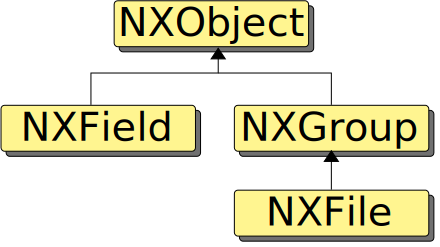
\includegraphics{pics/class_inheritance.pdf}}
\caption{{\small\label{fig:class_inheritance}
Inheritance relations between the major objects provided by \pninx.
\nxobject\ is the root of the class tree but will hardly be used. 
The class important to a developer are the three classes derived from 
\nxobject: \nxfield, \nxgroup, and \nxfile.
}}
\end{figure}
%%%----------------------------------------------------------------------------
To keep the API simple, only a few classes are exposed. These classes and their 
relationship among each other are depicted in Fig.~\ref{fig:class_inheritance}. 
The top-level class is \nxobject. It provides the common functionality 
of every object within the API. \nxfield\ and \nxgroup\ divide the classes 
available in two groups: the former class is the base for all data holding
objects while the latter is the fundamental container class. 
\nxgroup\ corresponds with some extensions to a group in an HDF5 file or to 
a directory in a file-system (if you like this picture more). 

\begin{description}
\item[\nxgroup] the standard container to hold all kinds of objects
\item[\nxfield] the data holding objects
\item[\nxfile] object representing a data file.
\end{description}
\nxfile is a descendant of \nxgroup\ as can be seen in
Fig.~\ref{fig:class_inheritance}. Thus it posses all the functionality that 
\nxgroup\ has aside from those methods necessary for file handling. 
\pninx\ uses HDF5 to write data to disk. However, you do not have to know 
anything about HDF5. No low level HDF5 calls are necessary. Everything is 
masked by the three objects mentioned above. 
In order to do so a Bridge pattern~\cite{book:gof} was used for the
implementation. The idea was to separate the interface provided to the user from the 
concrete interface used to communicate with the HDF5 library. 
This allows us to change the HDF5 backend completely without changing 
user code using the library (maybe recompilation is needed - but this is not as
bad as changing code). This gives us much more freedom in maintaining \pninx.
The bridge pattern is not implemented as shown in \cite{book:gof} but rather 
by using a template approach as shown  in \cite{book:alexandrescu}.
Hence the code remains free of pointers which makes it much more readable. 
Furthermore it should be mentioned that the \pninx\ heavily relies on features 
provided by the C++11 standard. Thus, an actual compiler is required to 
build the library (for {\tt gcc} a version larger or equal $4.4$ is required).
 

\section{A closer view on \nxfield}\label{section:nxfield_design}
The classes derived form \nxfield\ are most probably the most important 
objects in the \pninx-universe as they are used to read from and write data to 
the file. From the point of C++, \nxfield\ can be considered a container like 
{\tt std::vector<>} or {\tt std::list<>}.
When an \nxfield\ object is newly instantiated it represents an empty container. 
Writing data to disk means nothing else than appending data to the container. 
To read data form disk means to fetch data from the container.
The size (number of elements) of the container is limited by the amount of 
free space on the storage device on which the file is written.
This means that you do not know the number of elements you want to write 
at the time of instantiating these objects. 
All classes derived form \nxfield\ mimic the behavior of a C++ container 
class in some or the other way.  So you will find methods like 
{\tt get()}, {\tt set()}, {\tt append()} and so on. However, some flavors
of these method may behave slightly unexpected. The reason for this is that 
unlike for a classical container there are tow points of how we can look 
on the data stored in such a container (this is in particular true for 
numeric data). 
There are basically three kinds of objects that can be stored in these container
\begin{enumerate}
  \item numerical data (\nxnumericfield)
  \item strings (\nxstringfield)
  \item and binary uninterpreted data (\nxbinaryfield)
\end{enumerate}
\nxfield\ can handle all different kinds of data which keeps the number of 
classes in the library small. However, there is a price one has to pay 
for this simplicity: \nxfield\ behaves slightly different depending 
on which kind of data is stored. 

\subsection{Numerical data}
%%%-----------------------------------------------------------------------------
\begin{figure}[tb]
\centering
\begin{minipage}[t]{0.39\linewidth}
\centering
\resizebox{\linewidth}{!}{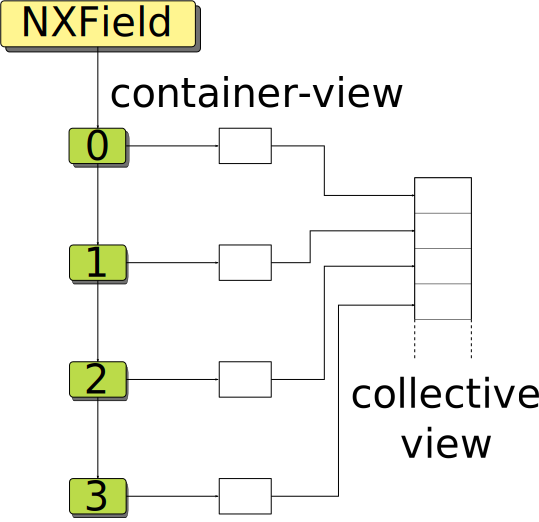
\includegraphics{pics/container_scalar.pdf}}
\caption{{\small\label{fig:container_scalar} An \nxfield\ object holding 
scalar values can be either considered as a list of single scalar values 
or as a 1-dimensional array of numbers.}}
\end{minipage}
\hfill
\begin{minipage}[t]{0.58\linewidth}
\centering
\resizebox{\linewidth}{!}{\includegraphics{pics/container_array.pdf}}
\caption{{\small\label{fig:container_array}An \nxfield\ object with 2D-arrays 
of data can be either considered as a list of individual arrays or as a
single 3D array where the first dimension runs over the number of elements
and the other dimension correspond to those of the array data.}}
\end{minipage}
\end{figure} 
%%%-----------------------------------------------------------------------------
Numeric data is handled by the two templates \arrayt\ and \scalart\  
provided by \pniutils. For more information on this two templates see 
the users-guide of \pniutils.
Figures~\ref{fig:container_scalar} and \ref{fig:container_array} show how these 
two templates are stored in a field container. 
Basically we can treat data in two different ways: as a list of invididual
elements or, collectively, as a single array of data. 
Both approaches are are depicted in Figs.~\ref{fig:container_scalar} and 
\ref{fig:container_array}. A field storing scalars can be either considered 
as a list of individual numbers or as a 1D array of numbers. 
The same holds for arrays as shown in Fig.~\ref{fig:container_array}. Here 
we have either a list of individual 2D arrays or a single 3D array where the 
first index runs over the number of elements in the list while the remaining 
indices correspond to those of the 2D arrays.
Both points of view - the element wise or the collective view have their own 
applications and thus are taken into account in the API. 

\subsection{String data}
%%%-----------------------------------------------------------------------------
\begin{figure}[tb]
\centering
\begin{minipage}[c]{0.4\linewidth}
\centering
\resizebox{\linewidth}{!}{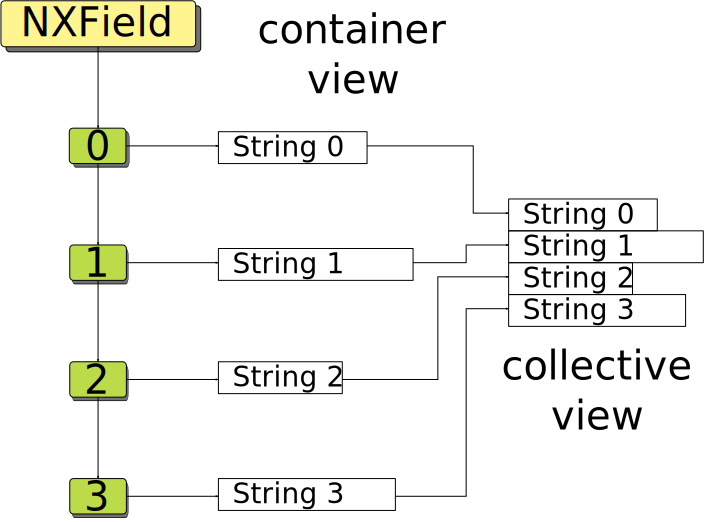
\includegraphics{pics/container_string.pdf}}
\end{minipage}
\hfill
\begin{minipage}[c]{0.58\linewidth}
\caption{{\small\label{fig:container_string} String fields can hold strings 
of different length. Each time a string is appended to the container 
a new entry is created. This can be used to store text files in a line-wise
manner. Each entry represents a line in the text-file.}}
\end{minipage}
\end{figure}
%%%-----------------------------------------------------------------------------
As usually strings are slightly different from everything else. 
This is also true for \pninx\ as shown in Fig.~\ref{fig:container_string}.
In the container view each element stores an individual string. The strings 
can have different length. 
As for numeric data one can either read individual strings or all strings 
in a single step. This would make it easy for instance to dump an entire 
ASCII file in such a string field. 

\subsection{Binary data}
%%%-----------------------------------------------------------------------------
\begin{figure}[tb]
\centering
\begin{minipage}[c]{0.4\linewidth}
\centering
\resizebox{\linewidth}{!}{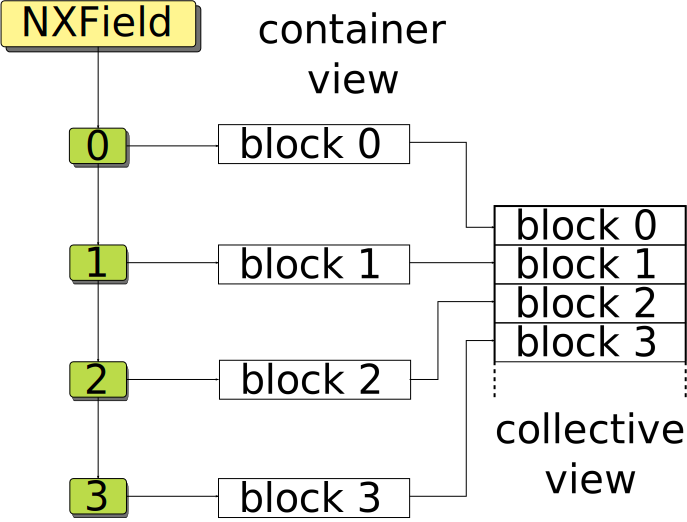
\includegraphics{pics/container_binary.pdf}}
\end{minipage}
\hfill
\begin{minipage}[c]{0.58\linewidth}
\caption{{\small\label{fig:container_binary} Binary data is stored block wise.
Each container entry holds a block of constant size of data. Thus at 
field creation a block size must be passed to the creating factory method. 
If the block size is as large as the entire binary data only a single element 
must be stored representing the entire binary data.}}
\end{minipage}
\end{figure}
%%%-----------------------------------------------------------------------------
The last class of data supported by Nexus is binary data. 
Image files (JPEG, PNG,TIFF), PDF files or other binary data can be stored in
such a field. The binary stream is not interpreted. 
The interesting question is how to represent such a binary blob of data in 
a container view as it is provided by \nxfield?. 
Binary data is usually read in blocks of a certain size. So the elements
in the list are blocks. In the simplest case a block is only $1$ byte. 
In this case you can read data byte by byte and dump it to the field. 




 



\chapter{Basic usage - the most important classes}\label{chapter:basic_usage}
%%low level objects in the library

\pninx s' API is quite minimalistic. From a users point of view only 
three classes are required: {\tt NXFile}, {\tt NXGroup}, and {\tt NXField}.
This are the basic components required to create a valid Nexus file and 
fill it with data. Each of this classes will be presented in a separate 
section of this chapter. 
Because using links takes a little more explanation this topic has 
its own section in at the very end of this chapter.

To start using \pninx\ you only need to include a single header file 
and maybe set a proper namespace
\begin{minted}[linenos=true]{c++}
#include<pni/nx/NX.hpp>

using namespace pni::nx::h5;
\end{minted}

The namespace selects which implementation to use. Actually only {\tt h5} for
HDF5 is supported.

\section{NXFile}\label{section:nxfile}
%%
{\tt NXFile} is the root for all data structures. 
Fortunately this class is also the simplest among the three {\tt NX} classes.
{\tt NXFile} is a descandent of {\tt NXGroup}, thus it exposes the full 
interface of {\tt NXGroup}. Since this will be the treated in the next 
section we will consider here only the file specific methods. 

For this purpose let's have a look on a simple example that already shows
everything we need to know in order to handle files. 
\lstinputlisting{../examples/c++/nxfile_ex1.cpp}
Lines 11-14 show the basic code sequence to create a new file. Setting 
overwrite to true (line 12) discardes an already existing file with the
same name. By default this option is not set in order to prevent a user 
from accidentaly overwritting existing files.
Once a file is opened or created any subsequent call to {\tt create()}, {\tt
setReadOnly} {\tt setOverwrite()}, or {\tt open()} will raise an  {\tt
NXFileError} exception.
The reason is that you must not change these attributes of the class 
while a file is open. First close the file object by invoking the 
{\tt close()} method. 

Once a file is created you may want to invoke its current status. 
This is shown in the next listing.
\lstinputlisting{../examples/c++/nxfile_ex2.cpp}
The interesting part of the code is shown in lines 16, 19, and 22.
The meaning of the methods shown in this lines is self explaining. 
All return bool values and are thus suitable for being used in 
conditional statements. 



\section{NXGroup}\label{section:nxgroup}
%%%documentation for NXGroup

\nxgroup\ is the fundamental object when it comes to structuring your file.
Everything what will be said about \nxgroup\ in this section holds for \nxfile\
too (it is a descendant of \nxgroup) too.
Groups are containers to hold \nxgroup\ or \nxfield\ objects.
Lets have a look on a simple example:

\inputminted[linenos=true]{c++}{../examples/c++/nxgroup_ex1.cpp}

A group is created using the {\tt create\_group} method provided by \nxgroup\ or
\nxfile\ objects (see lines 10-13). Several nested groups can be created using 
a single call as shown in line 13. The {\tt create\_group} method comes in 
two flavors: with one or with two arguments. In the former case the argument is
the path or name of the group and will simple create a group with that name
(path). The latter version of {\tt create\_group} takes the Nexus class 
of the group as a second argument. This method not only creates the group object
and attaches the {\tt NX\_class} attribute to it with a value determined by the 
second argument of the method.
Like all virtually all fundamental objects \nxgroup\ provides a {\tt close()}
method to close the object.
To open an existing group (this works for other objects too) you can either use
the {\tt open()} method of \nxgroup\ or \nxfile\ or the {\tt []} operator 
of these classes as shown in lines 16,17, and 20. In both cases the only
argument is the path to the group relative to the object that calls the method
or onto which the operator is applied. An absolute path can be used to access
objects which are located somewhere in the tree.

Although it is good practice to close all objects you have opened you do not

have to do so. As shown in this example too. When the objects loose scope they
become destroyed automatically. This is a good examples how using only first
class objects (no pointers to something) can improve code safety and simplicity.


\subsection{Working with attributes}

One of the most intriguing features of HDF5 and thus of Nexus is the concept of
attributes. Attributes are data-values that can be attached to every descendant
of \nxobject (which are \nxgroup, \nxfile, and \nxfield). An attribute can be considered basically pretty much like an 
\nxfield\ object although it has some limitations. It is, for instance, not
possible to grow a multidimensional attribute. Furthermore, attributes cannot be
compressed. 
The following examples gives a pretty good overview of what can be done with
attributes.
%%%--------------------------------------------------------------
\inputminted[linenos=true]{c++}{../examples/c++/nxgroup_ex2.cpp}
%%%--------------------------------------------------------------
The magic starts in line 15. An instance of \nxgroup\ is used to create a new
object of type \nxattribute. Such objects provide access to a particular
attribute. An instance of \nxattribute\ can be created using the {\tt attr<T>()}
template method provided by all classes derived from \nxobject.
The template parameters of this method determines the data-type to use for 
the attribute. In line 15 an attribute of type {\tt String} is created.
The only argument provided is a string with the name of the attribute. 
In this case a scalar attribute was created (one which holds only a single
value). In lines 16 and 19 the {\tt write} and {\tt read} methods of 
\nxattribute\ are used to write and read data to and from the attribute. 
Both methods are template so you should not case too much about the data type
you use for reading an writing such attribute as long as they are convertible. 
In lines 23 to 25 we do basically the same as before but for a {\tt Float32}
data-type. The interesting line here is 25. Here, a slightly different version
of the {\tt read} template method of \nxattribute\ is shown. Instead of passing
the target object to which the data should be read as an argument we tell the
method via a template parameter which object we would like to use to hold the
data. The method will then try to create such an object and returns it by value
to the calling program. As all objects in \pninx\ support move semantics you
should not care too much about performance issues in such a case. 

Until now we only created scalar attributes. In line 32 an array attribute is
created using the {\tt attr<T>()} template method. The template parameter again
determines the data-type to use for the attribute. However, to create an array
attribute we need to pass an additional argument to the method: the shape of the
array. In line 33 finally data is written to the attribute object.
Line 35 shows now the most elegant way how to obtain attribute data. Basically
we use the same {\tt read<T>()} template as in line 25 which does not only work
for primitive data-types but also for complex ones like arrays. 
The method does all the allocation and inquiry work us. We do not even specify
the type of the returned object (see left hand-side of the assignment operator).
Using {\tt auto} lets the decision up to the compiler. 

Now there are a few things left which one should to know about attributes. 
If you try to attach an attribute to an object which already posses an attribute
of same name an exception will be raised. However, this behavior can be
overridden by passing an additional argument to the attribute creation template
method telling the library to overwrite an already existing attribute. 
If one would like to use this feature line 23 of the above example must be
altered to 
\begin{minted}{c++}
    attr = g.attr<Float32>("temperature",true);
\end{minted}
where the last argument tells \pninx\ to overwrite an already existing attribute
of name {\tt temperature}. 
This works the same way for array attributes. Line 32 would change to
\begin{minted}{c++}
    attr = g.attr<UInt32>("vectors",wa.shape(),true);
\end{minted}
where again the last argument ensures that an already existing attribute would
be overwritten. 
It can be tedious to always use an instance of \nxattribute\ explicitly just to
write a simple attribute. So there is a simple shortcut for this. 
You can collate the code in lines 15 to 16 into
\begin{minted}{c++}
    g.attr<String>("description").write("a stupid data group");
\end{minted}

Finally the examples until now did not tell us anything how to obtain an
attribute from an already existing object. 
This can be done simply using the {\tt attr()} method provided by each object
(note that this method is not a template). It takes only one argument - the name
of the attribute. To open for instance the attribute from line 15 one would
simply type
\begin{minted}{c++}
    NXAttribute attr = g.attr("description"); 
\end{minted}
The method throws an exception if the attribute does not exist.





\section{NXField}\label{section:nxfield}
%%%NXField documentation

In the Nexus world the payload (your real data) is stored in fields which 
are represented in this library by objects of class {\tt NXField}.
Like groups, fields cannot be instantiated by their constructor but are 
rather created using factory methods provided by all classes derived 
from  {\tt NXGroup}. One word of caution: a prerequisit for understanding 
this section is a fundamental knowledge of the data objects provided 
by {\tt libpniutils}. If you are not please consult the {\tt libpniutils}
users guide first.
One can distinguish between two basic types of fields: string-fields
and numeric-fields. The former hold string data while the later 
holds numbers.   

\subsection{Creating fields}

The first step to use fields is to create them. Field creation for 
string and numeric fields is shown in this next example. 
\lstinputlisting{../examples/c++/nxfield_ex1.cpp}.
As we have seen in section~\ref{section:nxfield_design} the handling 
of data in \nxfield\ depends on the class of data that should be stored 




\subsection{Reading and writing numericaldata}
\label{section:nxfield_numeric_io}

\subsection{Reading and writing string data}
\label{section:nxfield_string_io}

\subsection{Reading and writing binary data}
\label{section:nxfield_binary_io}


\section{Links}\label{section:links}

\section{A full example}\label{section:full_example}


\chapter{Library configuration}
TO BE WRITTEN

\newpage
\addcontentsline{toc}{chapter}{Bibliography}
\bibliographystyle{ieeetr}
\bibliography{users-guide}

\end{document}
